\chapter{Equazione di Poisson}
	
\section{Caso unidimensionale}
		
	\noindent Consideriamo una classe di problemi al contorno
	\begin{equation}\label{eq:poisson-univ-gen}
		\begin{cases}
			-y'' (x) + q (x) y (x) = g (x) & x \in (\, a, b \,) \\
			y (a) = \alpha \\
			y (b) = \beta
		\end{cases}
	\end{equation}
	con \((\, a, b \,)\) limitato, \(q \in \cont ([\, a, b \,])\) tale che \(q (x) \ge 0\) per ogni \(x \in [\, a, b \,]\) e \(g \in \cont ([\, a, b \,])\).
	
	Studieremo in particolare il problema di Poisson univariato
	\begin{equation}\label{eq:poisson-univ}
		\begin{cases}
			-y'' (x) + c y (x) = f (x) & x \in (\, a, b \,) \\
			y (a) = 0 \\
			y (b) = 0
		\end{cases}
	\end{equation}
	con \((\, a, b \,)\) limitato, \(c > 0\) e \(f \in \cont ([\, a, b \,])\).
	
	Se si suppone che la soluzione \(y\) al problema in \eqref{eq:poisson-univ} appartenga a \(\cont^4 ([\, a, b \,])\), sviluppando in serie di Taylor centrate in \(x\), esistono \(\xi_1 \in (\, x, x + h \,)\) e \(\xi_2 \in (\, x - h, x \,)\) tali che
	\begin{align*}
		y (x + h) &= y (x) + h y' (x) + \frac{h^2}{2} y'' (x) + \frac{h^3}{6} y''' (x) + \frac{h^4}{24} y^{(4)} (\xi_1) \\
		y (x - h) &= y (x) - h y' (x) + \frac{h^2}{2} y'' (x) - \frac{h^3}{6} y''' (x) + \frac{h^4}{24} y^{(4)} (\xi_2)
	\end{align*}
	da cui, sommando membro a membro, esiste \(\xi \in (\, a, b \,)\) tale che
	\begin{equation*}
		y (x + h) + y (x - h) = 2 y (x) + h^2 y'' (x) + \frac{h^4}{12} y^{(4)} (\xi)
	\end{equation*}
	In base a ciò si giustifica l'approssimazione della derivata seconda con le \emph{differenze centrate}
	\begin{equation}\label{eq:poisson-diff-centr}
		y'' (x) \approx \frac{y (x + h) - 2 y (x) + y (x - h)}{h^2}
	\end{equation}

	A partire dalla \eqref{eq:poisson-diff-centr} si può discretizzare il problema \eqref{eq:poisson-univ} utilizzando le differenze centrate, ottenendo per ogni \(x \in (\, a, b \,)\)
	\begin{equation}\label{eq:poisson-discretizz}
		- \frac{y (x + h) - 2 y (x) + y (x - h)}{h^2} + c y (x) \approx - y'' (x) + c y (x) = f (x)
	\end{equation}
	e \(y (t) = 0\) per ogni \(x \notin (\, a, b \,)\).
	
	Considerando la discretizzazione equispaziata dell'intervallo \([\, a, b \,]\) definita da \(x_k = a + k h\) per \(k \in \Set{0, \dots, n + 1}\) con \((n + 1) h = b - a\), per la \eqref{eq:poisson-discretizz} si possono riscrivere le equazioni relativamente ai punti \(x_i\) e approssimare \(y (x_k)\) con \(u_k\) che risolvano il sistema di equazioni
	\begin{equation*}
		\forall k \in \Set{1, \dots, n} \colon - \frac{u_{k + 1} - 2 u_k + u_{k + 1}}{h^2} + c u_k = f (x_k)
	\end{equation*}
	con \(u_0 = u_{n + 1} = 0\), o equivalentemente
	\begin{equation}\label{eq:poisson-pre-matrice}
		\frac{1}{h^2} \qty(- u_{k + 1} + (2 + c h^2) u_k - u_{k - 1}) = f (x_k)
	\end{equation}
	La forma delle equazioni nella \eqref{eq:poisson-pre-matrice} permette di interpretarle matricialmente come \(A u = b\), con
	\begin{equation}\label{eq:poisson-matrice}
		A = \frac{1}{h^2}
		\begin{pmatrix}
			2 + c h^2 & - 1    & 0      & \cdots & 0         \\
			- 1       & \ddots & \ddots & \ddots & \vdots    \\
			0         & \ddots & \ddots & \ddots & 0         \\
			\vdots    & \ddots & \ddots & \ddots & -1        \\
			0         & \cdots & 0      & -1     & 2 + c h^2
		\end{pmatrix}
	\end{equation}
	e \(b_k = f (x_k)\) per ogni \(k \in \Set{1, \dots, n}\).
	
	\begin{esempio}
		Nel caso in cui \(n = 4\), le equazioni sintetizzate da \(A u = b\) sono
		\begin{equation*}
			\begin{cases*}
				\frac{1}{h^2} \qty[- u_2 + \qty(2 + c h^2) u_1 - \cancel{u_0}] = f (x_1) \\
				\frac{1}{h^2} \qty[- u_3 + \qty(2 + c h^2) u_2 - u_1] = f (x_2) \\
				\frac{1}{h^2} \qty[- u_4 + \qty(2 + c h^2) u_3 - u_2] = f (x_3) \\
				\frac{1}{h^2} \qty[- \cancel{u_5} + \qty(2 + c h^2) u_4 - u_3] = f (x_4)
			\end{cases*}
		\end{equation*}
		il che permette di intuire che, qualora \(u_0 = y (a) = \alpha\) e \(u_5 = y (b) = \beta\), il sistema da risolvere sarebbe \(A u = b\) con \(b_1 = f (x_1) + \alpha / h^2\) e \(b_n = f (x_n) + \beta / h^2\) quali unici valori modificati.
	\end{esempio}

	La matrice \(A\) descritta nella \eqref{eq:poisson-matrice} è simmetrica e, per i Teoremi~\ref{th:gerschgorin-1} e \ref{th:gerschgorin-3}, definita positiva, con lo spettro contenuto in \([\, c, c + 4 h^{-2} \,]\); dato che \(c > 0\), \(A\) è pure a predominanza diagonale stretta.
	
	\begin{table}[tpb]
		\centering
		
		\caption{Esempi di comportamento dello spettro di \(A\) al variare di \(n\), con \(c = 1\).}
		
		\begin{tabular}{S[table-format=2.0]%
				S[table-format=1.5e2]%
				S[table-format=2.4]%
				S[table-format=4.3]%
				S[table-format=1.3e1]%
				S[table-format=1.5e1]}
			\toprule
			{\(n\)} & {\(h\)} & {\(\lambda_{\textup{min}}\)} & {\(\lambda_{\textup{max}}\)} & {\(c + 4 h^{-2}\)} & {\(\kappa (A)\)} \\
			\midrule
			05 & 1.66667e-01 & 10.6462 & 135.354 & 1.450e+02 & 1.27139e+01 \\
			10 & 9.09091e-02 & 10.8027 & 475.197 & 4.850e+02 & 4.39888e+01 \\
			15 & 6.25000e-02 & 10.8379 & 1015.16 & 1.025e+03 & 9.36675e+01 \\
			20 & 4.76190e-02 & 10.8512 & 1755.15 & 1.765e+03 & 1.61747e+02 \\
			25 & 3.84615e-02 & 10.8576 & 2695.14 & 2.705e+03 & 2.48226e+02 \\
			30 & 3.22581e-02 & 10.8612 & 3835.14 & 3.845e+03 & 3.53106e+02 \\
			\bottomrule
		\end{tabular}
	\end{table}

	\begin{teorema}
		Se \(y\) è la soluzione di \eqref{eq:poisson-univ} e \(u_k \approx y (x_k)\) con \(x_k = a + k h\) per \(k \in \Set{0, \dots, n + 1}\) con \((n + 1) h = b - a\), allora
		\begin{equation}
			\frac{\norm{(u_i)_i - (y (x_k))_k}_2}{\sqrt{n}} = \order{h^2}
		\end{equation}
	
		Se, inoltre, la soluzione \(y\) è di classe \(\cont^4\) su \([\, a, b \,]\), allora
		\begin{equation}
			\norm{(u_i)_i - (y (x_k))_k}_\infty \le \frac{h^2}{24} \bigl\| y^{(4)} \bigr\|_\infty \, \norm{(x - a) (b - x)}_\infty
		\end{equation}
	\end{teorema}

	\begin{osservazione}
		Poiché la matrice \(A \in M_n (\R)\) della \eqref{eq:poisson-matrice} è tridiagonale, il sistema lineare \(A u = b\) può essere risolto mediante l'eliminazione gaussiana in \(\order{n}\) operazioni.
		
		Se il parametro \(c\) nella \eqref{eq:poisson-univ} è nullo, si può dimostrare che \(A\) è comunque definita positiva e che il suo spettro è contenuto in \([\, \delta, 4 h^{-2} \,]\), con \(\delta > 0\) indipendente da \(h\).
	\end{osservazione}

\section{Caso bidimensionale}
	
	\noindent Nel quadrato unitario  \(\varOmega = [\, 0, 1 \,] \times [\, 0, 1 \,]\), il problema di Poisson si configura come
	\begin{equation}\label{eq:poisson-quadrato}
		\begin{cases}
			\Delta u (x, y) = f (x, y) & (x, y) \in (\, 0, 1 \,) \times (\, 0, 1 \,) \\
			u (x, y) = g (x, y) & (x, y) \in \partial \varOmega
		\end{cases}
	\end{equation}
	ove
	\begin{equation*}
		\Delta u (x, y) = \pdv[2]{u}{x} + \pdv[2]{u}{y}
	\end{equation*}
	è il laplaciano di \(u\).
	
	Definita la griglia di punti \(\mathcal{G} = \Set{(x_i, y_j) | i, j \in \Set{0, \dots, n + 1}}\) con
	\begin{align*}
		h &= \frac{1}{n + 1} &
		x_i &= i h &
		y_j &= j h
	\end{align*}
	risulta evidente che, se almeno uno dei due indici \(i, j\) è o \(0\) o \(n + 1\), allora il punto \((x_i, y_j)\) è un punto del bordo e, per le condizioni in \eqref{eq:poisson-quadrato}, il valore della soluzione è ivi determinato. Resta da studiare, quindi, il valore della soluzione nei punti della griglia interni a \(\varOmega\).
	
	\begin{figure}[tpb]
		\centering
		
		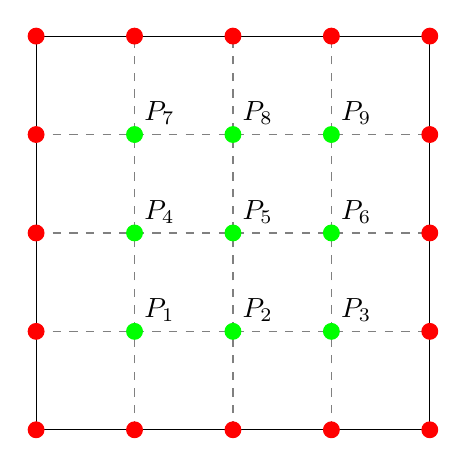
\begin{tikzpicture}[scale = 5]
			\draw (0, 0) -- (1, 0) -- (1, 1) -- (0, 1) -- cycle;
			\foreach \x in {0.25, 0.5, 0.75} {
				\draw[dashed, gray] (\x, 0) -- (\x, 1);
				\draw[dashed, gray] (0, \x) -- (1, \x);
			}
			
			\foreach \x in {0, 0.25, ..., 1} {
				\filldraw[red] (\x, 0) circle [radius = 0.2mm];
				\filldraw[red] (\x, 1) circle [radius = 0.2mm];
			}
			\foreach \x in {0.25, 0.5, 0.75} {
				\filldraw[red] (0, \x) circle [radius = 0.2mm];
				\filldraw[red] (1, \x) circle [radius = 0.2mm];
			}
		
			\foreach \x in {0.25, 0.5, 0.75} {
				\foreach \i in {0.25, 0.5, 0.75} {
					\filldraw[green] (\x, \i) circle [radius = 0.2mm];
				}
			}
		
			\node at (0.25,0.25) [above right] {\(P_1\)};
			\node at (0.25,0.50) [above right] {\(P_4\)};
			\node at (0.25,0.75) [above right] {\(P_7\)};
			\node at (0.50,0.25) [above right] {\(P_2\)};
			\node at (0.50,0.50) [above right] {\(P_5\)};
			\node at (0.50,0.75) [above right] {\(P_8\)};
			\node at (0.75,0.25) [above right] {\(P_3\)};
			\node at (0.75,0.50) [above right] {\(P_6\)};
			\node at (0.75,0.75) [above right] {\(P_9\)};
		\end{tikzpicture}
		
		\caption{Rappresentazione della griglia \(\mathcal{G}\) nel caso \(h = 1 / 4\). In verde sono segnati i punti in cui si vuole trovare il valore della soluzione, in rosso i punti al bordo, in cui la soluzione è nota.}\label{fig:poisson-quadrato-griglia}
	\end{figure}

	Supponendo che la soluzione \(u\) sia sufficientemente regolare, dalla formula di Taylor multivariata segue che
	\begin{multline*}
		u \qty(x + \tilde{h}, y + \tilde{k}) \approx u (x, y) + \tilde{h} \pdv{u (x, y)}{x} + \tilde{k} \pdv{u (x, y)}{y} \\
		+ \frac{\tilde{h}^2}{2} \pdv[2]{u (x, y)}{x} + \frac{\tilde{k}^2}{2} \pdv[2]{u (x, y)}{y} + \frac{\tilde{h} \tilde{k}}{2} \pdv[2]{u (x, y)}{x}{y}
	\end{multline*}
	Ponendo, quindi, \(\tilde{h} = \pm h\) e \(\tilde{k} = 0\) si trova
	\begin{align*}
		u (x + h, y) &\approx u (x, y) + h \pdv{u (x, y)}{x} + \frac{h^2}{2} \pdv[2]{u (x, y)}{x} \\
		u (x - h, y) &\approx u (x, y) - h \pdv{u (x, y)}{x} + \frac{h^2}{2} \pdv[2]{u (x, y)}{x}
	\end{align*}
	da cui
	\begin{equation}\label{eq:poisson-quadrato-x}
		u (x + h, y) + u (x - h, y) \approx 2 u (x, y) + h^2 \pdv[2]{u (x, y)}{x}
	\end{equation}
	e similmente, ponendo \(\tilde{h} = 0\) e \(\tilde{k} = \pm h\) si trova
	\begin{align*}
		u (x, y + h) &\approx u (x, y) + h \pdv{u (x, y)}{y} + \frac{h^2}{2} \pdv[2]{u (x, y)}{y} \\
		u (x, y - h) &\approx u (x, y) - h \pdv{u (x, y)}{y} + \frac{h^2}{2} \pdv[2]{u (x, y)}{y}
	\end{align*}
	da cui
	\begin{equation}\label{eq:poisson-quadrato-y}
		u (x, y + h) + u (x, y - h) \approx 2 u (x, y) + h^2 \pdv[2]{u (x, y)}{y}
	\end{equation}
	
	Riscrivendo la \eqref{eq:poisson-quadrato-x} e la \eqref{eq:poisson-quadrato-y} in modo da mettere in evidenza le derivate parziali seconde
	\begin{align*}
		\pdv[2]{u (x, y)}{x} &\approx \frac{u (x + h, y) - 2 u (x, y) + u (x - h, y)}{h^2} \\
		\pdv[2]{u (x, y)}{y} &\approx \frac{u (x, y + h) - 2 u (x, y) + u (x, y - h)}{h^2}
	\end{align*}
	si vede che è possibile approssimare il laplaciano di \(u\)
	\begin{multline}
		\Delta u (x, y) \approx \frac{1}{h^2} [u (x + h, y) + u (x - h, y) \\
		+ u (x, y + h) + u (x, y - h) - 4 u (x, y)]
	\end{multline}
	e, in particolare,
	\begin{multline*}
		\Delta u (x_i, y_j) \approx \frac{1}{h^2} [u (x_i + h, y_j) + u (x_i - h, y_j) \\
		+ u (x_i, y_j + h) + u (x_i, y_j - h) - 4 u (x_i, y_j)]
	\end{multline*}

	Sulla base di quest'ultima affermazione, la prima equazione del problema in \eqref{eq:poisson-quadrato} può essere approssimata con
	\begin{multline}\label{eq:poisson-quadrato-approx}
		u (x_{i + 1}, y_j) + u (x_{i - 1}, y_j) + u (x_i, y_{j + 1}) \\
		+ u (x_i, y_{j - 1}) - 4 u (x_i, y_j) = h^2 f (x_i, y_j)
	\end{multline}
	per ogni \(i, j \in \Set{1, \dots, n}\), mentre si ha \(u (x_i, y_j) = g (x_i, y_j)\) ogniqualvolta \(i \in \Set{0, n + 1}\) oppure \(j \in \Set{0, n + 1}\), dato che in tali casi il punto \((x_i, y_j)\) appartiene a \(\partial \varOmega\).
	
	\begin{figure}[tpb]
		\centering
		
		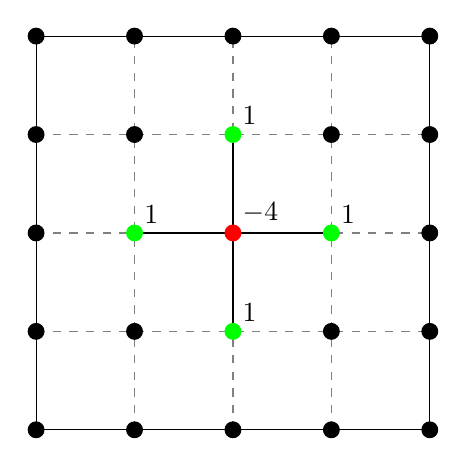
\begin{tikzpicture}[scale = 5]
			\draw (0, 0) -- (1, 0) -- (1, 1) -- (0, 1) -- cycle;
			\foreach \x in {0.25, 0.5, 0.75} {
				\draw[dashed, gray] (\x, 0) -- (\x, 1);
				\draw[dashed, gray] (0, \x) -- (1, \x);
			}
			
			\foreach \x in {0, 0.25, ..., 1} {
				\filldraw (\x, 0) circle [radius = 0.2mm];
				\filldraw (\x, 1) circle [radius = 0.2mm];
			}
			\foreach \x in {0.25, 0.5, 0.75} {
				\filldraw (0, \x) circle [radius = 0.2mm];
				\filldraw (1, \x) circle [radius = 0.2mm];
			}
			
			\foreach \x in {0.25, 0.75} {
				\foreach \i in {0.25, 0.75} {
					\filldraw (\x, \i) circle [radius = 0.2mm];
				}
			}
			
			\draw[thick] (0.5,0.75) -- (0.5,0.25) (0.25,0.5) -- (0.75,0.5);
			
			\filldraw[red] (0.5,0.5) circle[radius = 0.2mm] node [black, above right] {\(-4\)};
			\foreach \x in {0.25, 0.75} {
				\filldraw[green] (0.5, \x) circle [radius = 0.2mm] node [black, above right] {\(1\)};
				\filldraw[green] (\x, 0.5) circle [radius = 0.2mm] node [black, above right] {\(1\)};
			}
		\end{tikzpicture}
	
		\caption{“Molecola” della discretizzazione del laplaciano di centro \((1 / 2, 1 / 2)\) e \(h = 1 / 4\). Si ricordi di dividere per \(h^2\) il valore della molecola.}
	\end{figure}

	Per rendere piú chiaro il sistema, si può ricorrere a una sua rappresentazione matriciale. Definita la matrice \(B \in M_n (\R)\)
	\begin{equation*}
		B =
		\begin{pmatrix}
			-4     & 1      & 0      & \cdots & 0      \\
			1      & \ddots & \ddots & \ddots & \vdots \\
			0      & \ddots & \ddots & \ddots & 0      \\
			\vdots & \ddots & \ddots & \ddots & 1      \\
			0      & \cdots & 0      & 1      & -4
		\end{pmatrix}
	\end{equation*}
	e definito il termine noto \(b\) sommando i contribuiti di \(f\) e \(g\) in \eqref{eq:poisson-quadrato} e in \eqref{eq:poisson-quadrato-approx}, se si pone
	\begin{equation*}
		A =
		\begin{pmatrix}
			B       & \uno_n & \zero_n & \cdots & \zero_n \\
			\uno_n  & \ddots & \ddots  & \ddots & \vdots  \\
			\zero_n & \ddots & \ddots  & \ddots & \zero_n \\
			\vdots  & \ddots & \ddots  & \ddots & \uno_n  \\
			\zero_n & \cdots & \zero_n & \uno_n & B
		\end{pmatrix}
	\end{equation*}
	e \(u_{(j - 1)n + i} = u (x_i, y_j)\) per \(i, j \in \Set{1, \dots, n}\), si ricava che la \eqref{eq:poisson-quadrato-approx} è equivalente al sistema lineare \(A u = b\), che si può risolvere col metodo di Jacobi, col metodo di Gauss-Seidel oppure col metodo del gradiente coniugato.
	
	\begin{esempio}\label{eg:poisson-quadrato-3}
		Poniamoci nel caso \(h = 1 / 3\) e chiamiamo \(u_{i, j} = u (x_i, y_j)\) per semplicità. Per come sono definiti, i valori \(u_{0, j}\), \(u_{3, j}\), \(u_{i, 0}\) e \(u_{i, 3}\) sono noti, in quanto determinati dalla funzione \(g\). Gli altri casi, invece, sono da calcolare mediante la \eqref{eq:poisson-quadrato-approx}; vediamo questi casi singolarmente
		
		\begin{figure}[tpb]
			\centering
			
			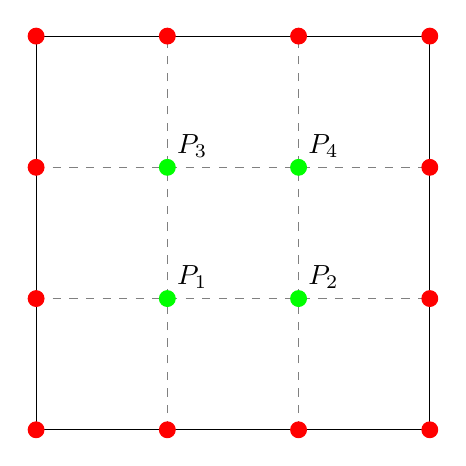
\begin{tikzpicture}[scale = 5]
				\draw (0, 0) -- (1, 0) -- (1, 1) -- (0, 1) -- cycle;
				\foreach \x in {1/3, 2/3} {
					\draw[dashed, gray] (\x, 0) -- (\x, 1);
					\draw[dashed, gray] (0, \x) -- (1, \x);
				}
				
				\foreach \x in {0, 1/3, 2/3, 1} {
					\filldraw[red] (\x, 0) circle [radius = 0.2mm];
					\filldraw[red] (\x, 1) circle [radius = 0.2mm];
				}
				\foreach \x in {1/3, 2/3} {
					\filldraw[red] (0, \x) circle [radius = 0.2mm];
					\filldraw[red] (1, \x) circle [radius = 0.2mm];
				}
				
				\foreach \x in {1/3, 2/3} {
					\foreach \i in {1/3, 2/3} {
						\filldraw[green] (\x, \i) circle [radius = 0.2mm];
					}
				}
				
				\node at (1/3,1/3) [above right] {\(P_1\)};
				\node at (2/3,1/3) [above right] {\(P_2\)};
				\node at (1/3,2/3) [above right] {\(P_3\)};
				\node at (2/3,2/3) [above right] {\(P_4\)};
			\end{tikzpicture}
			
			\caption{Griglia dell'Esempio~\ref{eg:poisson-quadrato-3}.}\label{fig:poisson-quadrato-esempio}
		\end{figure}
		
		\begin{description}
			\item[(\(i = 1\), \(j = 1\))] Si ha
			\begin{equation*}
				\begin{cases*}
					u_{2, 1} + u_{0, 1} + u_{1, 2} + u_{1, 0} - 4 u_{1, 1} = h^2 f (x_1, y_1) \\
					u_{0, 1} = g (x_0, y_1) \\
					u_{1, 0} = g (x_1, y_0)
				\end{cases*}
			\end{equation*}
			e, portando i termini noti tramite \(g\) al membro di destra, si ottiene
			\begin{equation*}
				u_{2, 1} + u_{1, 2} - 4 u_{1, 1} = h^2 f (x_1, y_1) - g (x_0, y_1) - g (x_1, y_0)
			\end{equation*}
			\item[(\(i = 2\), \(j = 1\))] Si ha
			\begin{equation*}
				\begin{cases*}
					u_{3, 1} + u_{1, 1} + u_{2, 2} + u_{2, 0} - 4 u_{2, 1} = h^2 f (x_2, y_1) \\
					u_{3, 1} = g (x_3, y_1) \\
					u_{2, 0} = g (x_2, y_0)
				\end{cases*}
			\end{equation*}
			e, portando i termini noti tramite \(g\) al membro di destra, si ottiene
			\begin{equation*}
				u_{1, 1} + u_{2, 2} - 4 u_{2, 1} = h^2 f (x_2, y_1) - g (x_3, y_1) - g (x_2, y_0)
			\end{equation*}
			\item[(\(i = 1\), \(j = 2\))] Si ha
			\begin{equation*}
				\begin{cases*}
					u_{2, 2} + u_{0, 2} + u_{1, 3} + u_{1, 1} - 4 u_{1, 2} = h^2 f (x_1, y_2) \\
					u_{0, 2} = g (x_0, y_2) \\
					u_{1, 3} = g (x_1, y_3)
				\end{cases*}
			\end{equation*}
			e, portando i termini noti tramite \(g\) al membro di destra, si ottiene
			\begin{equation*}
				u_{2, 2} + u_{1, 1} - 4 u_{1, 2} = h^2 f (x_1, y_2) - g (x_0, y_2) - g (x_1, y_3)
			\end{equation*}
			\item[(\(i = 2\), \(j = 2\))] Si ha
			\begin{equation*}
				\begin{cases*}
					u_{3, 2} + u_{1, 2} + u_{2, 3} + u_{2, 1} - 4 u_{2, 2} = h^2 f (x_2, y_2) \\
					u_{3, 2} = g (x_3, y_2) \\
					u_{2, 3} = g (x_2, y_3)
				\end{cases*}
			\end{equation*}
			e, portando i termini noti tramite \(g\) al membro di destra, si ottiene
			\begin{equation*}
				u_{1, 2} + u_{2, 1} - 4 u_{2, 2} = h^2 f (x_2, y_2) - g (x_3, y_2) - g (x_2, y_3)
			\end{equation*}
		\end{description}
	
		Ora poniamo
		\begin{equation*}
			b =
			\begin{pmatrix}
				b_1 \\
				b_2 \\
				b_3 \\
				b_4
			\end{pmatrix}
			=
			\begin{pmatrix}
				h^2 f (x_1, y_1) - g (x_0, y_1) - g (x_1, y_0) \\
				h^2 f (x_2, y_1) - g (x_3, y_1) - g (x_2, y_0) \\
				h^2 f (x_1, y_2) - g (x_0, y_2) - g (x_1, y_3) \\
				h^2 f (x_2, y_2) - g (x_3, y_2) - g (x_2, y_3)
			\end{pmatrix}
		\end{equation*}
		ordiniamo i punti secondo l'ordine lessicografico mostrato nella Figura~\ref{fig:poisson-quadrato-esempio}
		\begin{align*}
			P_1 &= (x_1, y_1) &
			P_2 &= (x_2, y_1) \\
			P_3 &= (x_1, y_2) &
			P_4 &= (x_2, y_2)
		\end{align*}
		e infine definiamo
		\begin{equation*}
			u =
			\begin{pmatrix}
				u (P_1) \\
				u (P_2) \\
				u (P_3) \\
				u (P_4)
			\end{pmatrix}
			=
			\begin{pmatrix}
				u_{1, 1} \\
				u_{2, 1} \\
				u_{1, 2} \\
				u_{2, 2}
			\end{pmatrix}
		\end{equation*}
		Si ottiene cosí il sistema \(A u = b\) equivalente alla \eqref{eq:poisson-quadrato-approx}, con
		\begin{equation*}
			A =
			\begin{pmatrix}
				B & \uno_2 \\
				\uno_2 & B
			\end{pmatrix}
			=
			\begin{pmatrix}
				-4 & 1  & 1  & 0  \\
				1  & -4 & 0  & 1  \\
				1  & 0  & -4 & 1  \\
				0  & 1  & 1  & -4
			\end{pmatrix}
		\end{equation*}
		ovvero il sistema di equazioni
		\begin{equation*}
			\begin{cases*}
				u_{2, 1} + u_{1, 2} - 4 u_{1, 1} = b_1 \\
				u_{1, 1} + u_{2, 2} - 4 u_{2, 1} = b_2 \\
				u_{2, 2} + u_{1, 1} - 4 u_{1, 2} = b_3 \\
				u_{1, 2} + u_{2, 1} - 4 u_{2, 2} = b_4
			\end{cases*}
		\end{equation*}
	\end{esempio}

\section{Stima dell'errore}
	
	\begin{teorema}
		Se \(u^*\) è la soluzione di \eqref{eq:poisson-quadrato} ed è di classe \(\cont^4\) in \(\varOmega\) e \(u_h\) è l'approssimazione di \(u^*\) ottenuta col metodo delle differenze a cinque punti relativamente alla griglia \(\mathcal{G} = \Set{(x_i, y_j) | i, j \in \Set{0, \dots, n + 1}}\) con
		\begin{align*}
			h &= \frac{1}{n + 1} &
			x_i &= i h &
			y_j &= j h
		\end{align*}
		allora
		\begin{subequations}
		\begin{equation}
			\abs{u^* (x_i, y_j) - u_h (x_i, y_j)} \le c h^2
		\end{equation}
		ove
		\begin{equation}
			c = \frac{1}{24} \qty(\max_{(x, y) \in \varOmega} \abs{\pdv[4]{u^* (x, y)}{x}} + \max_{(x, y) \in \varOmega} \abs{\pdv[4]{u^* (x, y)}{y}})
		\end{equation}
		\end{subequations}
	\end{teorema}